\section{Verificación de \textit{software} y funcionalidad}
\label{sec:verificacion}

La verificación es un paso esencial en el desarrollo de cualquier producto \textit{software}, ya que permite determinar la adecuación de las características diseñadas e implementadas en código a los requerimientos originalmente determinados para ellas y, además, discernir cuáles son los puntos en los que la especificación original difiere con el producto obtenido con el fin de poder subsanar las diferencias.

La importancia que tiene la verificación del \textit{software} ha auspiciado la aparición de un sinfín de metodologías, técnicas y formatos para ejecutar pruebas sobre el \textit{software}. Si bien no se aplican metodologías específicas de \textit{testing} durante esta evolución, cabe reseñar que se implementan y emplean activamente múltiples tipos de pruebas, tanto automáticas como manuales.

\subsection{Pruebas automáticas}
\label{subsec:pruebasAutomaticas}
En el contexto del presente proyecto, las pruebas automáticas son todas las pruebas implementadas en código que pueden ser ejecutadas a través del sistema de integración continua ante modificaciones del código volcadas en el sistema de control de versiones. El sistema de integración continua empleado ---véase \referenciaSeccion{subsec:cicd}--- está configurado adecuadamente para ejecutar la batería completa de las pruebas automáticas introducidas en los componentes servidor y extensión del proyecto. 

Las pruebas codificadas hacen uso de dependencias o librerías específicamente creadas con el fin de verificar que los resultados obtenidos al ejecutar una determinada pieza de código coinciden con los resultados esperados. Estas pruebas basan su funcionamiento en aserciones, que determinan cuál es el resultado esperado y lo comparan con el resultado obtenido; y en dobles, que son objetos utilizados en sustitución de las dependencias empleadas para agilizar las pruebas, simulando con exactitud el comportamiento que estas dependencias tendrían en un escenario real.

Según su alcance, se distinguen dos tipos fundamentales de pruebas automáticas implementadas en el presente proyecto: las pruebas \textbf{unitarias}, que buscan verificar el funcionamiento de bloques de código ---una función, una clase o un módulo--- de forma rápida y sencilla; y las pruebas de \textbf{integración}, que son aquellas que verifican cómo se produce la interacción entre funciones, clases o módulos dentro de un mismo componente.

Se introduce a continuación un análisis de las pruebas realizadas en el servidor y en la extensión de \textit{VSCode4Teaching}.

\subsubsection{\textit{Testing} del servidor}
Como la \referenciaSeccion{subsec:tecServidor} recoge, el servidor está basado en el \textit{framework} Spring y hace uso de \textbf{JUnit} como librería para la creación y ejecución de las pruebas en código relativas al servidor.

Haciendo uso de esta librería, se introducen en este componente dos tipos de pruebas unitarias:
\begin{itemize}
    \item \textit{Tests} de controladores. Dado un contexto en el que se definen las variables necesarias para poder ejecutar la funcionalidad verificada, se lanza una petición al servidor y se coteja la respuesta recibida a la petición con la respuesta esperada, comprobando la información de interés contenida tanto en la cabecera como en el cuerpo de la respuesta.
    \item \textit{Tests} de servicios. Definido el conjunto de las variables necesarias, estas pruebas verifican el correcto funcionamiento de los servicios implementados, que son la capa que alberga la lógica de negocio y que actúa como intermediaria entre los controladores y los repositorios ---siendo estos la puerta de enlace hacia el sistema de persistencia---.
\end{itemize}

A los tipos anteriores se suman los \textit{tests} de integración, que verifican el correcto funcionamiento del componente en su integridad. Para ello, se especifican una serie de variables para definir el contexto de la prueba y se lanza una llamada a un \textit{endpoint}, de modo que se ejecuta el procedimiento completo de invocación a la lógica de negocio y a la persistencia de base de datos para devolver al usuario la respuesta solicitada del mismo modo en que se haría en un contexto de ejecución real, sin sustituir ninguna de las capas por comportamientos simulados, verificando que la interrelación de los distintos paquetes del código funciona correctamente.

Acerca de la cantidad de pruebas implementadas, cabe reseñar que, previamente al inicio de la ejecución de los requisitos comprendidos en el presente Trabajo Fin de Grado, este componente contaba con un total de 80 \textit{tests} implementados; cantidad que se ha visto incrementada hasta las 96 pruebas en el momento de su finalización. La \referenciaFigura{fig:testsServidorIDE} refleja la ejecución satisfactoria de la batería de pruebas implementada dentro del entorno de desarrollo.

\begin{figure}[ht]
    \centering
    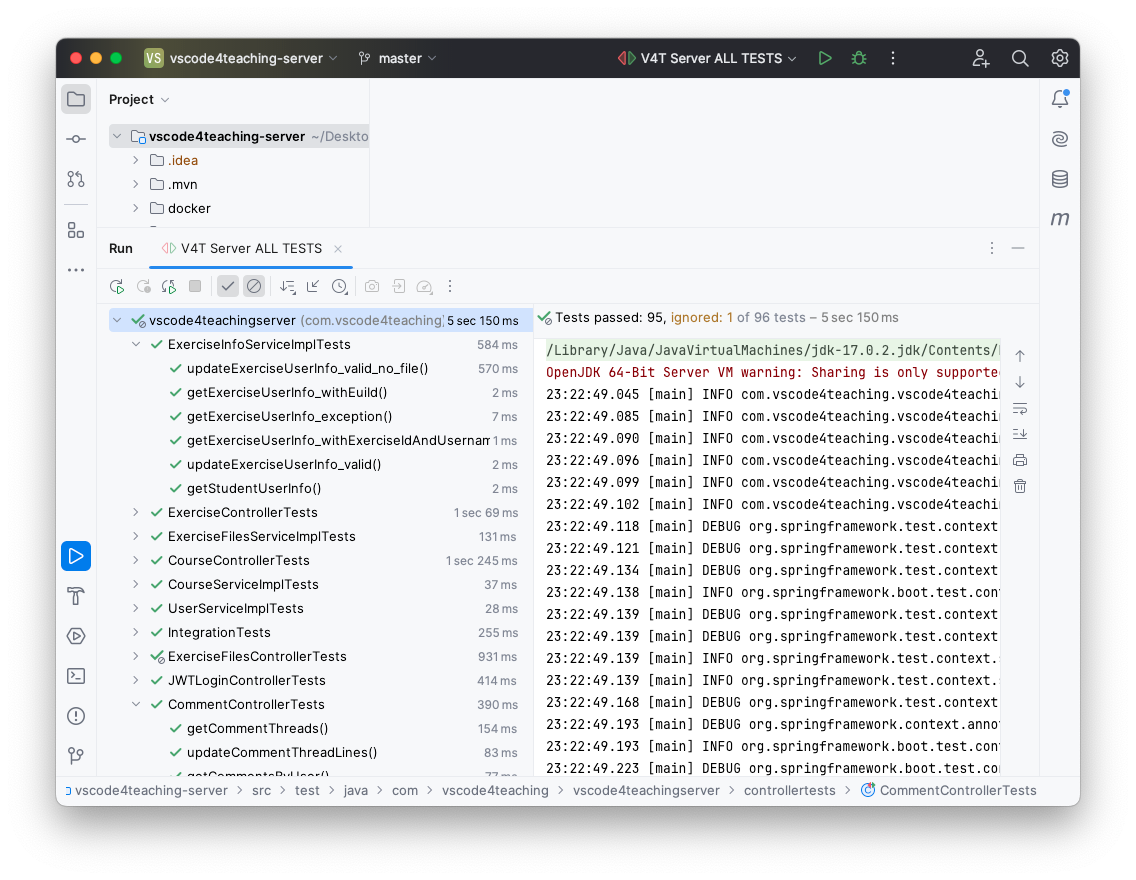
\includegraphics[width=\textwidth]{imagenes/utilizadas/4-4-verificacion/testsServidor.png}
    \caption{Instantánea de \textit{IntelliJ IDEA} mostrando el resultado satisfactorio de la ejecución de las pruebas del servidor.}
    \label{fig:testsServidorIDE}
\end{figure}

Una de las métricas aplicables para valorar la idoneidad o adecuación de las pruebas implementadas al componente realizado es la cobertura del código, que refleja en formato porcentual cuántas líneas o bloques de código han sido revisados por alguna de las pruebas automáticas ejecutadas. En la \referenciaFigura{fig:coberturaServidorFinal} se puede visualizar el informe de cobertura elaborado para el servidor en el momento de la finalización del trabajo. Para este componente, la cobertura de código es del 78,3\% de las clases, el 79,4\% de los métodos y el 77,6\% de las 1180 líneas de código que lo conforman; tasas elevadas que, pese al incremento en el tamaño del componente, permanecen en el mismo orden que al comienzo del proyecto.

\begin{figure}[ht]
    \centering
    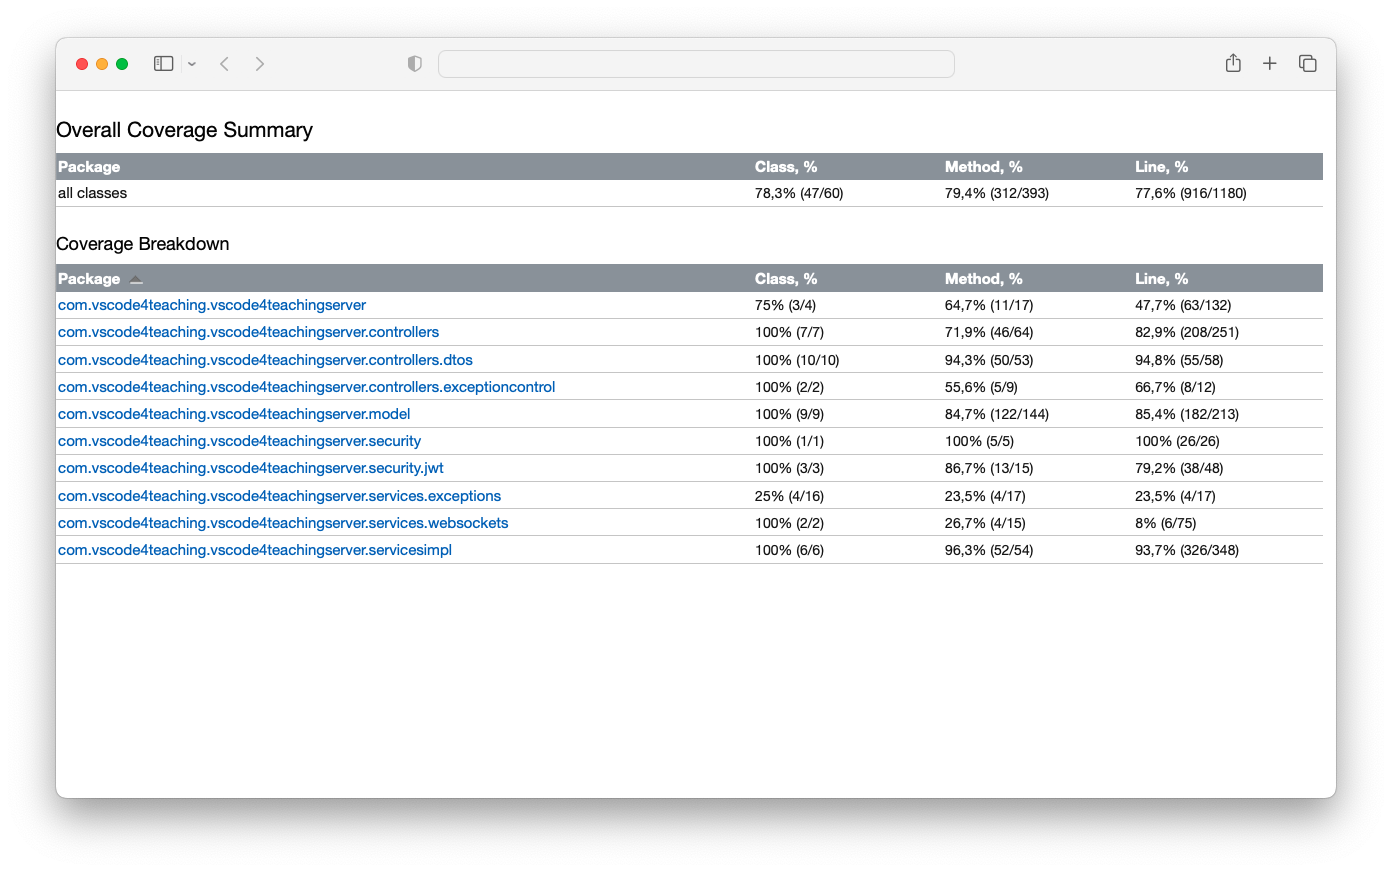
\includegraphics[width=\textwidth]{imagenes/utilizadas/4-4-verificacion/coverageServidorFinal.png}
    \caption{Informe de cobertura de las pruebas automáticas sobre el código del servidor.}
    \label{fig:coberturaServidorFinal}
\end{figure}

\subsubsection{\textit{Testing} de la extensión}
Análogamente al caso anterior, y tal como queda plasmado en la \referenciaSeccion{subsec:tecCliente}, la extensión emplea \textbf{Jest} como librería para la implementación de los \textit{tests} de este componente.

Previamente al inicio de la ejecución de los requisitos comprendidos en el presente Trabajo Fin de Grado, el proyecto contaba con un total de 97 \textit{tests} implementados, alcanzando la cifra de 129 pruebas en el momento de su finalización. La \referenciaFigura{fig:testsClienteIDE} incluye una visualización del entorno de desarrollo una vez terminada la ejecución exitosa de las pruebas implementadas en este componente.

\begin{figure}[ht]
    \centering
    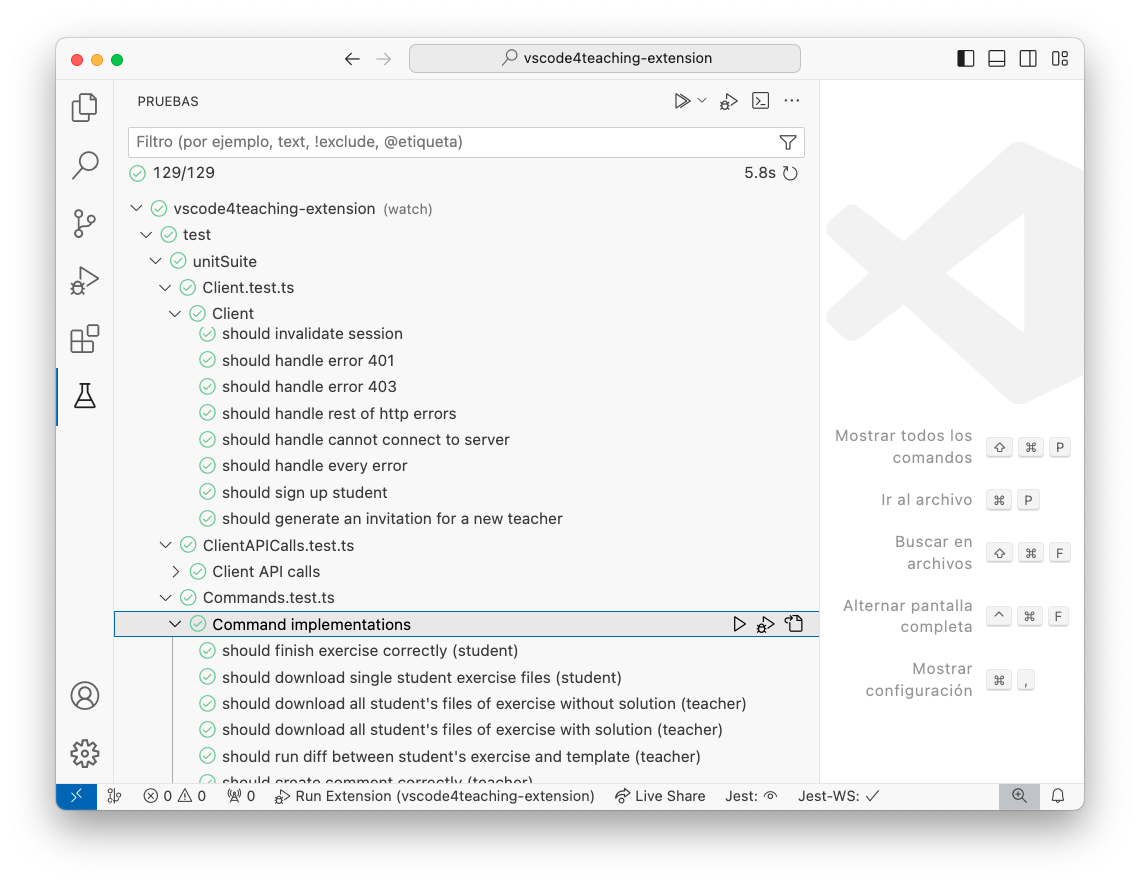
\includegraphics[width=\textwidth]{imagenes/utilizadas/4-4-verificacion/testsCliente.png}
    \caption{Captura de Visual Studio Code tras ejecutar las pruebas implementadas sobre la extensión.}
    \label{fig:testsClienteIDE}
\end{figure}

La \referenciaFigura{fig:coberturaExtensionFinal} introduce el informe de cobertura correspondiente a la extensión en el momento de la finalización del trabajo. En este punto, la cobertura alcanza cifras del 52,08\% de las funciones y el 60,1\% de las 1649 líneas del código generado. Estas tasas se mantienen en el mismo orden que al comienzo del proyecto, poniendo así de manifiesto que se han generado nuevas pruebas para cubrir adecuadamente todos los requisitos implementados y expandido otras anteriormente existentes en el proyecto.

\begin{figure}[ht]
    \centering
    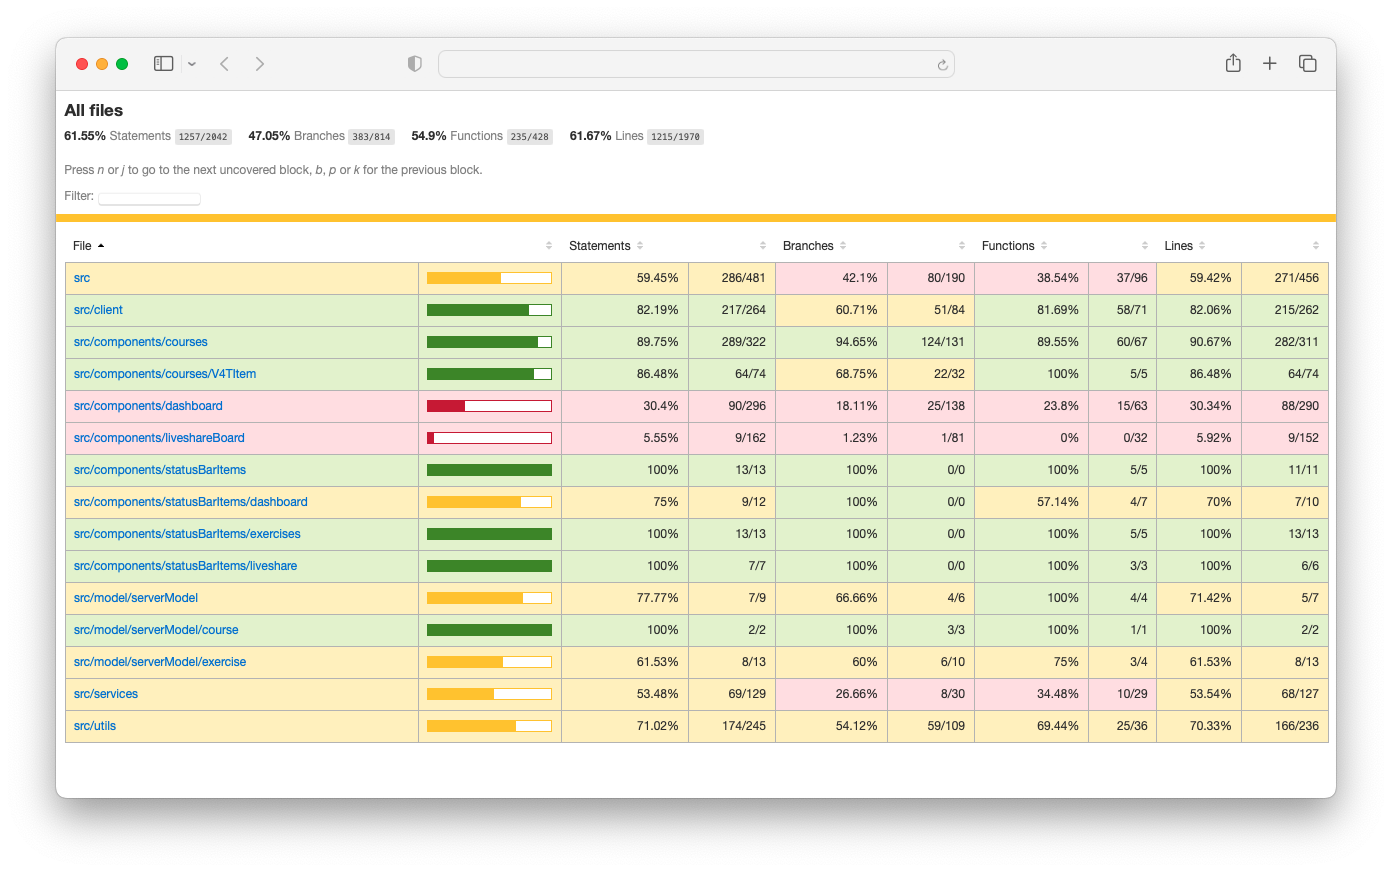
\includegraphics[width=\textwidth]{imagenes/utilizadas/4-4-verificacion/coverageExtensionFinal.png}
    \caption{Informe de cobertura de las pruebas automáticas sobre el código de la extensión para Visual Studio Code.}
    \label{fig:coberturaExtensionFinal}
\end{figure}

\subsection{Pruebas manuales}
\label{subsec:pruebasManuales}
Las pruebas implementadas en código no permiten simular el comportamiento impredecible propio de los usuarios finales de las aplicaciones, de modo que, si bien es posible automatizar pruebas que traten de emular la interacción con el usuario, no es viable fingir un uso real de la aplicación, que se caracterizará por la libertad que estos pueden ejercer en el uso de las funcionalidades de las que dispone el \textit{software} desarrollado.

Para tratar de suplir esta carencia, otro tipo de pruebas realizadas sobre el \textit{software} son las pruebas de \textbf{aceptación de usuario}, en las que una muestra de los usuarios finales acceden a una versión en \textit{pre-producción}, es decir, a una versión que incorpora todas las novedades que se pretende incluir en la nueva evolución del \textit{software} pero divulgada específicamente al grupo acotado de usuarios en régimen de pruebas. De ese modo, los probadores pueden ejecutar una serie de acciones para buscar y detectar errores que puedan escapar a las técnicas de verificación mediante \textit{tests} unitarios o de integración. Adicionalmente, como el proyecto no introduce pruebas de \textbf{rendimiento} o \textbf{carga} automáticas, se aprovecha la ejecución de estas pruebas para evaluar parámetros y detectar errores de estas características.

Durante el presente Trabajo Fin de Grado se han ejecutado pruebas de aceptación de usuario en tres ocasiones, dos de ellas previas al lanzamiento de las versiones más significativas ---véase la \referenciaSeccion{sec:distribDespliegue}--- y una adicional entre las dos anteriores. Las pruebas se han realizado en entornos que simulaban situaciones reales, contando con en torno a cuatro usuarios concurrentes de la extensión que empleaban un mismo servidor de \textit{VSCode4Teaching} desplegado mediante Docker en la red local a la que todos ellos estaban conectados, obteniendo los \textit{logs} registrados de todos los componentes y usuarios para disponer de una traza suficiente para analizar en busca de errores de interacción cliente-servidor en caso de producirse.

La utilidad de este formato de prueba queda confirmada gracias a requisitos de corrección de errores como el \texttt{RE-3} o \texttt{RE-5}, que fueron descubiertos gracias a estas pruebas de aceptación de usuario, permitiendo detectar la fuente del error para proceder con su triaje, tal como se detalla en la \referenciaSeccion{subsec:reqsErrores}. Estas pruebas no solo han servido para detectar y corregir errores: el formato de simulación de entorno real con usuarios potencialmente finales permite obtener realimentación directa del grupo de muestra empleado para introducir requisitos que, bajo su punto de vista, permitan mejorar la usabilidad y comprensibilidad de la aplicación. Prueba de ello es el requisito \texttt{RF-11} ---detallado en la \referenciaSeccion{subsec:rf11}---, por el que se introducen iconos de colores en la barra lateral para expresar información adicional en un solo vistazo, agilizando la interacción del usuario con la aplicación. Estas pruebas han permitido, además, corregir el error asociado al requisito \texttt{RE-6}, por el que se descubrió un problema relativo a la carga de trabajo del servidor, que a menudo era incapaz de procesar todas las peticiones enviadas por los clientes en un mismo instante a la hora de realizar subidas masivas de plantillas y propuestas de resolución de ejercicios por parte de los docentes, tal como queda detallado en la \referenciaSeccion{subsec:reqsErrores}.
